\chapter{강의 1: 끈 이론의 주요 주제}

\lectureoverview{환원주의에 대한 도전은 \(1+1\)차원에서의 보손화, 전기--자기 이중성, D-브레인, 강결합 전이, 창발하는 기하, 그리고 끈 진공의 조합론적 지형을 통해 한층 선명해진다. 동일한 물리계도 근본적으로 서로 다른 기본 기술로 설명될 수 있으며, 어떤 기술이 단순해 보이는지는 결합과 기하에 달려 있다.}

\section{환원주의, 복잡성, 그리고 단순성의 문제}

서스킨드는 일부러 익숙한 철학적 구호로 강의를 시작한다. 큰 것은 작은 것들로 이루어지고, 작은 것은 더 작은 것들로 이루어진다는 것이다. 이어 같은 생각의 더 야심 찬 형태, 즉 근본 물리학에서 정말 중요한 주장을 덧붙인다. 더 깊은 층위로 내려갈수록 대상은 작아질 뿐 아니라 더 단순해져야 한다는 것이다. 그는 집은 벽돌로 지어지며 아무도 집을 벽돌로 착각하지 않는다고 비유한다. 벽돌은 더 작지만 더 단순하기도 하다.

강의의 첫 단계는 이러한 기대를 입자물리학의 실제 상황과 대조하는 것이다. 환원주의가 이 강한 의미에서 점점 더 큰 단순성을 가져다준다면, 오늘날의 소립자 물리학은 간결한 모습에 가까우리라 기대할 수 있다. 그러나 서스킨드는 양자중력이 등장하기도 전에 이미 장부가 복잡해 보인다고 강조한다. 강의에서 제시한 수치는 대략적인 값이지만, 그 대략성 자체가 논점의 일부다:
\begin{equation}
\begin{aligned}
N_{\mathrm{species}}&\sim 75,\\
N_{\mathrm{independent}}&\sim 10\text{--}20,\\
N_{\mathrm{parameters}}&\sim 20.
\end{aligned}
\end{equation}
이것으로 이야기가 끝나는 것도 아니다. 표준 모형에는 중력이 없고, 암흑 물질을 설명하지 못하며, 인플레이션에 필요한 추가 구조도 제공하지 않고, 심각한 미세 조정 문제도 안고 있다. 통상적인 보완 기제를 더하면 수는 오히려 늘어난다. 강의에서는 초대칭을 예로 든다. 강의 당시 많은 물리학자는 대형 강입자 충돌기가 초대칭 짝입자를 드러내기를 기대했다. 서스킨드는 그에 따른 확장이 장부를 곧바로 단순화하기는커녕 매개변수를 백 개 넘게 추가한다고 강조한다. 그의 개략적인 요지는 다음과 같다.
\begin{equation}
N_{\mathrm{parameters}}^{\mathrm{extended}} \sim 200.
\end{equation}
이 수치들은 의도적으로 대략적이며 당시의 상황을 반영한다. 더 깊은 기술이라고 해서 입자 목록과 측정된 상수의 관점에서 반드시 더 단순해 보이는 것은 아니라는 주장을 뒷받침하는 데 쓰인다.

이러한 정량적 불만은 아직 서스킨드의 핵심 논지가 아니다. 이는 서론이다. 더 깊은 주장이자 강의의 나머지를 이끄는 주장은 현대 양자장론과 끈 이론이 벽돌과 집을 유일하고 결합과 무관하게 구분할 수 있음을 뚜렷하게 뒷받침하지 않는다는 것이다. 이어지는 예들은 ``기본적''이라는 말의 의미 자체가 어떤 변수가 효율적인지에 달려 있을 수 있음을 보여주기 위해 선택되었다.

\section{보손화: 고정된 근본성의 첫 번째 붕괴}

서스킨드가 드는 첫 이론적 예는 \(1+1\)차원 양자장론, 즉 공간 한 차원과 시간 한 차원의 이론이다. 그는 자세한 동치 유도는 하지 않겠다고 먼저 밝힌다. 여기서 중요한 것은 형식적 증명이 아니라 개념적 교훈이다.

페르미온 장론에서 시작하자. 페르미온 장은 \(\psi\)로 표기한다. 가까이 있는 두 페르미온은 보손 복합체를 이룰 수 있으며, 그에 대응하는 보손 장은 \(\phi\)로 표기한다. 얼핏 보면 위계는 분명해 보인다. \(\psi\)은 기본이고 \(\phi\)는 복합 변수 또는 유효 변수다. 강의에서는 보손을 페르미온 결합쌍을 생성하는 장으로 정확히 이런 식으로 도입한다.

그러나 같은 이론을 정반대의 출발점에서 다시 쓸 수 있다는 사실이 발견되었다. 보손 장 \(\phi\)에서 시작할 수 있으며, 그러면 페르미온은 더 이상 점 모양의 구성 요소로 나타나지 않는다. 대신 보손 장의 킨크로 나타난다. 이는 \(\phi\)이 두 점근값 사이를 매끄럽게 보간하는 확장된 배치다. 강의에서 제시하는 최소한의 수학적 내용은 이 점근 구조다:
\begin{equation}
\phi(x\to -\infty)=\phi_-,
\qquad
\phi(x\to +\infty)=\phi_+.
\end{equation}
이를 나타내는 편리한 개략적 형태는 다음과 같다.
\begin{equation}
\phi(x)\approx \frac{\phi_++\phi_-}{2}
+
\frac{\phi_+-\phi_-}{2}\tanh\!\left(\frac{x}{\ell}\right),
\end{equation}
여기서 \(\ell\)는 전이 영역의 폭이다.

\editorialnote{쌍곡탄젠트 형태는 강의에서 그린 킨크를 나타내는 표준적인 매끄러운 예이지, 강의에서 유도한 공식은 아니다. 정확한 보손화 대응 사전은 모형에 따라 다르다. 개념의 핵심은 페르미온 여기와 보손 장의 위상 솔리톤 사이의 교환이다.}

강의에서 든 벨트 비유는 그대로 살려 둘 만큼 정확하다. 꼬임이 없는 평평한 벨트는 킨크가 없는 배치다. 벨트 한쪽 끝을 \(2\pi\)만큼 회전시키면, 멀리 떨어진 곳에서는 벨트가 같은 국소 방향으로 돌아오지만, 중간에는 확장된 꼬임 영역을 지나야 한다. 그 꼬임 영역이 킨크다. 보손 기술에서는 페르미온이 바로 이런 확장된 대상으로 표현된다.

결합을 도입하면 요점이 더욱 분명해진다. 서스킨드는 이 예에서 결합을 \(G\)라고 부른다. 두 기술이 막연히 관련되어 있다는 말이 아니라, 각 기술의 효율성이 매개변수 영역에 달려 있다는 뜻이다.
\begin{align}
G \ll 1
&\Rightarrow
\ell\text{ small, tight kink; }\psi\text{ efficient},\\
G \gg 1
&\Rightarrow
\ell\text{ large, broad kink; }\phi\text{ efficient}.
\end{align}
\(G\)가 작으면 킨크는 좁고 페르미온은 단순한 대상으로 보인다. \(G\)가 커질수록 킨크는 넓어지고 페르미온은 점 모양에서 멀어진다. 그러면 보손 변수가 더 간결한 기술이 된다.

\paragraph{개략적 갱신 규칙}
\begin{enumerate}
\item 페르미온 장론 \(\psi\)에서 시작한다.
\item 보손 복합체를 식별하고 이를 \(\phi\)로 기술한다.
\item 같은 이론을 전적으로 \(\phi\)만으로 다시 쓴다.
\item 보손 기술에서는 페르미온이 폭 \(\ell\)인 킨크로 다시 나타난다.
\item \(G\ll 1\)일 때 \(\ell\)는 작고 페르미온 기술이 가장 간결하다.
\item \(G\)가 더 커지면 \(\ell\)가 커지고 보손 기술이 가장 간결해진다.
\end{enumerate}

이는 고정된 ``집과 벽돌'' 관점에 대한 첫 번째 명시적 반례다. 강의의 요점은 단순히 복합체가 존재한다는 것이 아니라, 무엇을 기본 변수로 보느냐가 결합에 따라 달라질 수 있다는 데 있다.

\section{전하, 자기 단극자, 약결합과 강결합}

이어서 서스킨드는 더 익숙한 입자물리학에도 비슷한 이야기가 있는지 묻는다. 예로 드는 것은 전하와 자기 단극자의 관계다. 이 용어법에서 전자 같은 보통의 하전 입자는 전기 단극자, 즉 전기장의 국소적 원천이다. 자기 단극자는 막대자석 비유로 도입한다. 보이지 않는 연결 막대 없이 막대자석의 한쪽 끝만 어떻게든 떼어 낼 수 있다면, 그 끝의 장선은 전하의 장선과 정확히 같은 모양이되 전기장이 아니라 자기장일 것이다.

관련 제어 매개변수는 미세 구조 상수 \(\alpha\)다. 강의에서 서스킨드는 이를 전하의 제곱으로 발견적으로 다룬다.
\begin{equation}
\alpha \sim e^2.
\end{equation}
또한 대략적인 조작적 해석도 제시한다. 이 상수는 전자가 얼마나 쉽게 복사하는지를 나타내며, 강의에서는 그 세기를 관련된 의미에서 가속된 전자가 대략 ``\(1/100\)''개의 광자를 방출한다고 요약한다. 강의에서 사용한 대략적인 수치로는 다음과 같다.
\begin{equation}
\alpha \approx 10^{-2}.
\end{equation}
이는 정밀한 관례를 제시하려는 것이 아니라 전기적 결합이 약함을 설명하기 위한 교육적 표현이다.

\editorialnote{약결합--강결합 관계는 디랙 양자화에 정확한 선례가 있다. 흔히 쓰이는 관례 가운데 하나에서는 전기 전하와 자기 전하가 \(e g_m=2\pi n\)를 만족한다. 따라서 약한 전기 결합은 강한 자기 결합에 대응하지만, 정확한 수치 인자와 보호되는 질량 관계는 이론에 따라 달라진다.}

\(\alpha\ll 1\)일 때 전자는 단순한 대상이다. 전기장은 약하고 진공 편극 구름은 희박하며, 전자는 거의 점처럼 보인다. 반대로 자기 단극자는 장이 엄청나고 주변이 심하게 뒤틀리며, 크고 복잡하고 무겁다. 서스킨드는 이 상황을 약결합--강결합의 관점에서 다음과 같이 요약한다.
\begin{equation}
\begin{aligned}
\alpha \ll 1
&\Rightarrow \text{simple electron;}\\
&\phantom{\Rightarrow{}}\text{heavy, extended monopole},\\
\alpha \gg 1
&\Rightarrow \text{simple monopole;}\\
&\phantom{\Rightarrow{}}\text{heavy, structured electron}.
\end{aligned}
\end{equation}
강의에서는 단극자의 질량 공식을 유도하지 않는다. 그럴 필요도 없다. 요점은 정성적이다. \(\alpha\)가 커지면 전자의 장은 강해지고 구조는 커지는 한편, 단극자는 작아지고 가벼워진다. 단위보다 훨씬 큰 영역에서는 유용한 기술이 서로 뒤바뀐다. 단극자는 단순해지고 전자는 복잡해진다.

이는 앞서 보손화에서 얻은 교훈을 장론의 맥락에서 보여준다. 기본적인 것과 복합적인 것의 구분은 절대적이지 않다. 결합에 달려 있다.

\begin{classroomqa}
\audiencequestion{환원주의가 믿을 만한 길잡이가 아니라면, 계를 임의로 작은 조각으로 나누는 것처럼 보이는 미적분학을 물리학자들은 왜 사용하는가? \lecturetimestamp{00:21:21}}
\lecturerresponse{미적분학은 연속적인 변화를 전제하지만 이론의 근본 대상을 식별하지는 않는다. 양자장은 모든 거리 척도에서 요동하므로, 무엇이 기본인지 최종적으로 한 번에 결정할 수 있는 매끄러운 층위가 아니라 끝없는 위계를 만들어 낸다.}
\end{classroomqa}

이어서 그 위계가 프랙털과 비슷하다는 제안이 나온다. 서스킨드는 그 비유를 받아들이면서 한층 분명히 한다. 양자장은 모든 척도에서 요동하므로 고전적인 의미에서는 결코 매끄럽지 않다. 이러한 과도한 변화는 양자장론을 수학적으로 어렵게 만드는 요인 중 하나다. 보통의 미적분학을 적용할 때는 순진하게 매끄러운 미시적 장이 아니라 재규격화된 양을 사용해야 한다.

\section{끈, D-브레인, 그리고 약결합--강결합 이중성의 귀환}

강의의 다음 전환은 일부러 순진한 생각에서 시작한다. 끈 이론이 근본 구성 요소의 이론이라면 답은 간단할 것이다. 구성 요소는 끈이다. 서스킨드는 이런 기대를 숨김없이 말한 다음, 강의의 다음 부분에서 이를 하나씩 무너뜨린다.

\subsection{끈이 모든 것을 설명하지는 않는 이유}

첫 번째 복잡성은 D-브레인이 불가피하게 존재한다는 점이다. D\(p\)-브레인은 끈이 끝날 수 있는 \(p\)차원 대상이다. 문자 \(D\)는 디리클레 경계 조건에서 왔지만, 이름보다 그 역할이 훨씬 중요하다. 이 대상들은 이론의 일부이므로 버릴 수 없다. 선택적으로 덧붙이는 장식물이 아니다.

가장 간단한 예는 다음과 같다.
\begin{itemize}
\item 점 모양인 D0-브레인,
\item 끈 모양인 D1-브레인, 즉 D-끈,
\item 보통의 기본 끈인 F-끈.
\end{itemize}
D0-브레인은 임의의 수의 F-끈이 끝날 수 있는 무거운 점 모양의 자리다. D1-브레인은 무거운 케이블 같은 대상으로, F-끈보다 훨씬 굵고 단위 길이당 질량이 크지만 이 역시 F-끈이 끝날 수 있는 곳이다. 강의에서는 약결합에서 이들을 동등하게 기본적인 대안으로 제시하지 않는다. D-브레인은 무겁고 구조가 있으며 복합체처럼 보이지만, 이론에서 배제할 수 없는 대상으로 소개된다.

\editorialnote{이 강의 부분에서 다루는 홀수 차원 브레인 이론은 IIB형 끈 이론이다. 여기서 안정한 D-브레인은 공간 차원이 홀수이며, D1-브레인과 D3-브레인을 포함한다. 서스킨드는 분류보다 이중성의 양상이 당면한 주제이므로 이러한 명칭의 설명을 뒤로 미룬다.}

\paragraph{표기법}
서스킨드는 강의의 여러 부분에서 \(G\)와 \(g\)를 다소 느슨하게 사용한다. 여기서는 \(G\)를 보손화 예에 한정하고, \(g\)는 끈 결합을 나타낸다.

끈 결합 \(g\)는 공리적으로가 아니라 조작적으로 정의된다. 요동하는 끈이 분열하여 딸끈을 만드는 확률을 나타내는 매개변수다. 그래서 서스킨드는 이를 QED에서 \(\alpha\)가 하는 역할과 직접 비교한다. 강의에서는 잠시 멈추어 장력과 단위 길이당 에너지가 같다는 점도 설명한다.
\begin{equation}
T=\frac{E}{L}=\frac{M}{L}.
\end{equation}

F-끈과 D-끈의 표준 장력 공식은 약결합--강결합 비교를 명시적으로 보여준다.
\begin{equation}
T_{\mathrm{F1}}=\frac{1}{2\pi\alpha'},
\qquad
T_{\mathrm{D1}}=\frac{1}{2\pi\alpha' g_s},
\qquad
\frac{T_{\mathrm{D1}}}{T_{\mathrm{F1}}}=\frac{1}{g_s}.
\end{equation}
\editorialnote{이 장력 공식은 강의의 케이블과 실 비유에 사용된 통상적인 정규화를 제시한다. 이는 편집 과정에서 추가한 내용이며, 강의에서는 결합에 따른 스케일링만 사용한다.}

\subsection{F-끈과 D-끈}

이어서 끈의 언어로 약결합--강결합 이야기가 되풀이된다. 결합이 작을 때 F-끈은 가볍고 가늘어 기본 대상에 대한 직관적인 원래 모습에 가깝다. D-끈은 굵고 무거우며 F-끈 구조로 가득하다. 결합이 커질수록 F-끈은 더 쉽게 분열한다. 그 주위에 딸끈 구름이 늘어나면서 F-끈은 더 무겁고 복잡해진다. 동시에 이제 무거워진 F-끈을 방출하기가 D-끈에 점점 더 어려워지므로, 주변 구조는 희박해지고 D-끈은 더 가볍고 선 모양에 가까워진다. 따라서 강의의 약결합--강결합 대응은 다음과 같다.
\begin{align}
g \ll 1
&\Rightarrow
\begin{gathered}
\text{F-string light and thin;}\\
\text{D-string heavy and structured},
\end{gathered}\\
g \sim 1
&\Rightarrow
\text{F-string and D-string comparable},\\
g \gg 1
&\Rightarrow
\begin{gathered}
\text{D-string light and thin;}\\
\text{F-string heavy and structured}.
\end{gathered}
\end{align}
서스킨드는 \(g\sim 1\) 부근에서는 두 기술이 뚜렷이 구분되지 않게 된다고 말한다. 그 지점을 넘어서면 두 기술의 역할이 사실상 서로 바뀐다. 이것은 전자--단극자 교환에 해당하는 끈 이론의 현상이며, 통용되는 명칭은 S-이중성이다.

끈이 고리로 닫힌 뒤에도 같은 교환을 살펴볼 수 있다. 약결합에서는 작은 F-끈 고리가 가벼운 입자 같은 여기인 반면, 이에 대응하는 D-끈 고리는 무겁고 복잡하다. 강결합에서는 역할이 뒤집힌다. D-끈 고리가 가벼운 기술이 되며, 그 결과 생기는 가벼운 닫힌끈 여기 가운데 중력자가 있다. 강의는 익숙한 입자의 정체성조차 이중성의 어느 쪽을 사용하는지에 달릴 수 있음을 강조하려고 이 예를 든다.

강의는 여기서 한 걸음 더 나아간다. 이상화된 이론에서 결합은 손으로 조정하는 숫자에 그치지 않고 장처럼 거동한다. 개략적으로는 다음과 같다.
\begin{equation}
g = g(x).
\end{equation}
따라서 공간의 서로 다른 영역에서 서로 다른 쌍대 기술이 유리할 수 있다. 한 영역에서는 F-끈이 가벼운 변수이고, 다른 영역에서는 D-끈이 가볍다. 그 사이에서는 특별히 단순한 것이 없다. 그래서 서스킨드에게 끈 이론은 단순한 환원주의 관점을 되살리는 것이 아니다. 오히려 그 모호성을 극단으로 밀어붙인다.

\editorialnote{섭동 끈 이론에서 국소 결합은 딜라톤 \(g_s(x)=e^{\Phi(x)}\)으로 정해진다. 따라서 \(g=g(x)\)라고 쓰는 것은 단순한 비유가 아니다. 다만 현실적인 콤팩트화에서는 대체로 이러한 변화를 제한하는 퍼텐셜이 생긴다.}

\begin{classroomqa}
\audiencequestion{다른 영역에서 결합이 충분히 변해 D-끈이 F-끈보다 가벼워진다면 관측 가능한 스펙트럼에도 변화가 생기는가? \lecturetimestamp{00:34:15}}
\lecturerresponse{그렇다. 이것이 논의 중인 정확히 대칭적이고 수학적으로 제어된 모형을 우리 세계와 직접 동일시할 수 없는 이유 중 하나다. 여기서 얻는 교훈은 일관된 양자 이론이 어떤 현상을 보일 수 있는가에 관한 것이지, 자연의 스펙트럼을 그대로 나타내는 것은 아니다.}
\end{classroomqa}

\begin{classroomqa}
\audiencequestion{D2-브레인에도 이에 대응하는 쌍대 기술이 있는가? \lecturetimestamp{00:34:39}}
\lecturerresponse{있다. 하지만 D-끈과 비슷한 또 다른 교환은 아니다. 짝수 차원 브레인의 경우에는 막으로 해석하고 추가 공간 차원을 도입하게 되며, 이것이 다음 구성이다.}
\end{classroomqa}

\begin{classroomqa}
\audiencequestion{끈이 분열할 확률이 커지면 내부 구조도 더 복잡해지는가? \lecturetimestamp{00:34:53}}
\lecturerresponse{그렇다. 작동 원리를 구체적으로 보려면 QED로 돌아가자. 전자가 광자를 방출하고, 광자는 하전 입자쌍으로 요동하며, 그 하전 선들은 다시 복사한다. 결합이 커지면 이 위계는 덜 희박해진다.}
\end{classroomqa}

\subsection{질문을 계기로 양자전기역학으로 돌아가다}

그러자 학생이 분열 확률이 커지면 단순히 구조가 더 복잡해지는 것인지 묻는다``.'' 서스킨드는 양자전기역학으로 돌아가 전자의 세계선을 다시 그려 답한다. 이 회귀가 중요한 이유는 끈에 관한 이야기가 별개의 기묘한 사례가 아니라 같은 약결합--강결합 양상의 또 다른 예임을 보여주기 때문이다.

\begin{figure}[htbp]
\centering
\begin{tikzpicture}[scale=1.0]
\draw[->] (-1.2,0) -- (3.7,0) node[right] {space};
\draw[->] (0,-0.2) -- (0,4.3) node[above] {time};

\draw[line width=0.9pt] (0,0.2) -- (0,4.0);
\node[left] at (0,3.55) {\(e^{-}\)};

\draw[line width=0.8pt] (0,1.0) -- (0.18,1.08) -- (0.36,0.92) -- (0.54,1.10) -- (0.72,0.94) -- (0.90,1.12) -- (1.08,0.96) -- (1.26,1.14);
\draw[line width=0.8pt] (0,2.35) -- (-0.18,2.43) -- (-0.36,2.27) -- (-0.54,2.45) -- (-0.72,2.29) -- (-0.90,2.47);

\draw[line width=0.8pt] (1.26,1.14) -- (1.48,1.42);
\draw[line width=0.8pt] (1.26,1.14) -- (1.04,1.42);
\draw[line width=0.8pt] (1.48,1.42) -- (1.58,2.10);
\draw[line width=0.8pt] (1.04,1.42) -- (0.94,2.10);
\draw[line width=0.8pt] (0.94,2.10) -- (1.58,2.10);

\draw[line width=0.7pt] (1.58,1.78) -- (1.72,1.84) -- (1.86,1.72) -- (2.00,1.86);
\draw[line width=0.7pt] (0.94,1.78) -- (0.80,1.84) -- (0.66,1.72) -- (0.52,1.86);

\node at (2.35,1.95) {\(\gamma\)};
\node at (-1.15,2.75) {\(\gamma\)};
\end{tikzpicture}
\caption{강의에서 사용한 QED 위계의 개략도: 점 전자가 광자를 방출하고, 광자가 입자쌍을 만들며, 딸 하전 선들이 다시 복사하여 점점 더 짧은 척도에 구조를 만들어 낸다.}
\end{figure}

강의의 요점은 점 전자에도 일련의 과정이 뒤따른다는 것이다.
\begin{enumerate}
\item 전자는 광자를 방출하고 흡수한다.
\item 광자는 전자--양전자 쌍을 만들 수 있다.
\item 딸 하전 선들도 광자를 방출할 수 있다.
\item 이 위계는 더 작은 척도까지 이어진다.
\end{enumerate}
결합이 약하면 이 구름은 희박하므로 실험실에서는 전자가 거의 점처럼 보인다. 결합이 강해지면 구조가 증식하여 전자는 구조를 가진 대상으로 변한다. 이어 끈 이야기는 이를 직접 비유하는 사례로 제시된다.

이후의 같은 논의는 서스킨드의 발견적 에너지 장부도 설명해 준다. 관련 에너지는 자유 입자의 기여를 단순히 합한 값이 아니라고 그는 강조한다. 상호작용 에너지도 포함해야 한다.
\begin{equation}
E_{\mathrm{tot}} = E_e + E_\gamma + E_{\mathrm{int}}.
\end{equation}
여기서 \(E_{\mathrm{int}}\)가 핵심 항이다. 이 항이 있어야 옷 입은 전자의 질량에 주변 장과 가상 구조에 관련된 에너지가 포함된다. 강의에서는 이를 형식적인 재규격화 자기 에너지 유도로 다루지 않는다. 요점은 발견적이지만 핵심적이다. 대상의 질량에는 그 주위의 복잡한 구름을 지탱하는 데 필요한 상호작용 에너지가 이미 포함되어 있다.

\begin{classroomqa}
\audiencequestion{전자가 실제 쌍을 만들 자유 에너지를 충분히 갖고 있지 않다면, 가상 광자와 전자--양전자 쌍을 만드는 에너지는 어디서 오는가? \lecturetimestamp{00:37:01}}
\lecturerresponse{맨전자에서 시작해 나중에 쿨롱 장을 덧붙이는 식으로 생각하지 않는다. 관측되는 전자는 옷 입은 상태이며, 그 질량에는 장 에너지와 상호작용 에너지가 이미 포함되어 있다. QED에서 전체 에너지는 자유 전자 에너지와 자유 광자 에너지만의 합이 아니다. 상호작용 항은 필수적이다. 중간 상태의 쌍을 가상이라고 부르는 것은 유용하지만, 에너지 장부는 상호작용하는 전체 상태에 속한다.}
\end{classroomqa}

\begin{classroomqa}
\audiencequestion{고에너지 탐침이 이 구조를 드러낼 때, 탐침이 이미 존재하던 것을 발견한 것이 아니라 구조를 만들어 낸 것인가? \lecturetimestamp{00:38:59}}
\lecturerresponse{그 해석상의 구분은 논쟁의 여지가 있다. 조작적으로는 충분히 높은 에너지의 산란에서 계산 가능한 비자명한 최종 상태가 나온다. 약결합에서는 대부분의 사건이 여전히 단순해 보이지만, 대략 \(\alpha\) 정도의 비율로 추가 복사나 쌍이 드러난다.}
\end{classroomqa}

\begin{classroomqa}
\audiencequestion{D1-브레인이 F-끈보다 더 무겁다고 할 때, 그 장력도 더 큰가? \lecturetimestamp{00:39:37}}
\lecturerresponse{그렇다. 확장된 끈에서 ``질량''은 여기서 단위 길이당 에너지를 뜻하며, 이는 바로 장력이다.}
\end{classroomqa}

\begin{figure}[htbp]
\centering
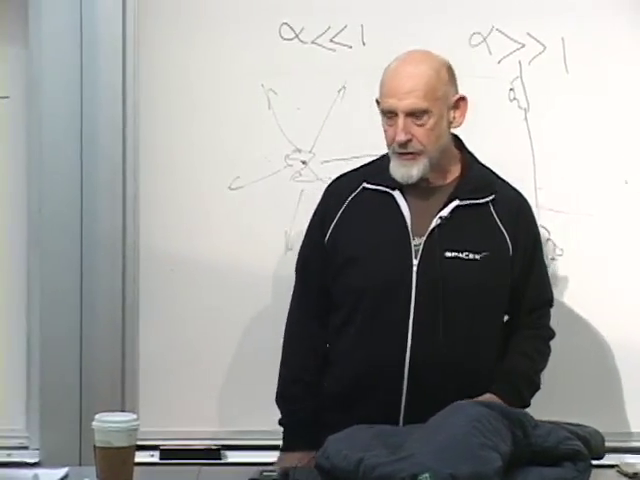
\includegraphics[width=0.72\textwidth]{lecture_01_figure_02.png}
\lectureframe{00:38:22.500}

\vspace{1em}

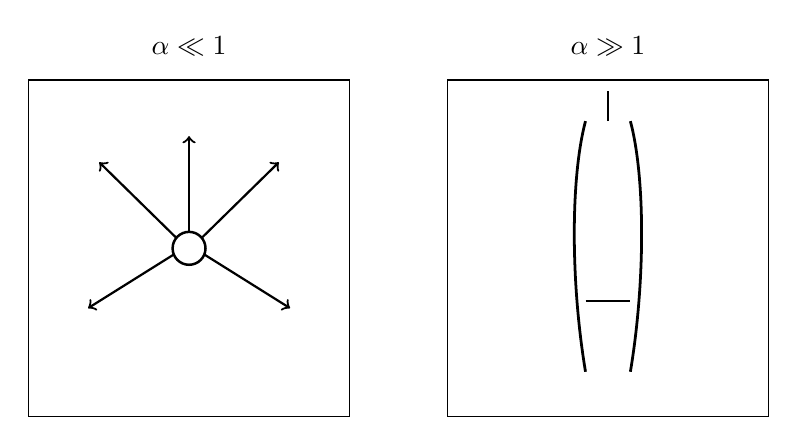
\begin{tikzpicture}[scale=0.95]
\draw (-5.3,-2.4) rectangle (-1.0,2.1);
\draw (0.3,-2.4) rectangle (4.6,2.1);

\node at (-3.15,2.55) {$\alpha \ll 1$};
\node at (2.45,2.55) {$\alpha \gg 1$};

\draw[line width=0.9pt] (-3.15,-0.15) circle (0.22);
\draw[->,line width=0.8pt] (-3.15,0.07) -- (-3.15,1.35);
\draw[->,line width=0.8pt] (-2.98,-0.01) -- (-1.95,1.00);
\draw[->,line width=0.8pt] (-3.32,-0.01) -- (-4.35,1.00);
\draw[->,line width=0.8pt] (-2.95,-0.23) -- (-1.80,-0.95);
\draw[->,line width=0.8pt] (-3.35,-0.23) -- (-4.50,-0.95);

\draw[line width=1.0pt] (2.15,-1.8) .. controls (1.95,-0.6) and (1.95,0.8) .. (2.15,1.55);
\draw[line width=1.0pt] (2.75,-1.8) .. controls (2.95,-0.6) and (2.95,0.8) .. (2.75,1.55);
\draw[line width=0.8pt] (2.15,-0.85) -- (2.75,-0.85);
\draw[line width=0.8pt] (2.45,1.55) -- (2.45,1.95);
\end{tikzpicture}
\caption{상호작용 에너지 논의에서 다룬 QED의 약결합--강결합 비교. 이 그림은 서스킨드가 설명하는 두 영역, 즉 희박한 약결합 구름과 증식하는 강결합 구름을 따로 보여준다.}
\end{figure}

약결합--강결합 비교가 앞서 도입되었는데도 이 그림이 여기에 놓인 이유는, 강의에서 서스킨드가 상호작용 에너지와 구조의 증식을 논하는 이 질문 중심의 대목에서 대조를 다시 그리기 때문이다.

\section{짝수 차원 브레인 이론과 창발하는 추가 차원}

여기까지 강의는 페르미온과 보손, 전자와 단극자, F-끈과 D-끈 사이의 교환을 강조해 왔다. 다음 단계는 더 놀랍다. 서스킨드는 홀수 차원 브레인 대신 짝수 차원 D-브레인을 갖는 다른 끈 이론으로 전환한다. 이 구분이 중요한 까닭은 이 이론에는 F-끈과 교환할 D-끈이 없기 때문이다. 여기에는 D0-브레인, D2-브레인, D4-브레인 등이 있다.

따라서 강결합 극한은 한 끈을 다른 끈으로 이름만 바꿔 부르는 것일 수 없다. 강의에 따르면 더 기묘한 일이 벌어진다. 추가 공간 차원이 뚜렷하게 드러난다. 서스킨드는 먼저 이를 가장 극적인 표현으로 말한다 --- ``새 차원이 모습을 드러낸다'' ---. 그리고 곧바로 더 신중한 진술로 바꿔 설명한다. 아주 작은 콤팩트 방향이 무시할 수 없을 때까지 커진다는 것이다.

장부를 맞추는 일도 논점의 일부이므로, 서스킨드는 여기서 잠시 멈춘다.
\begin{equation}
\begin{aligned}
10\text{-dimensional string theory} &= 9\text{ space}+1\text{ time},\\
11\text{-dimensional theory} &= 10\text{ space}+1\text{ time}.
\end{aligned}
\end{equation}
강의의 주장은 짝수 차원 브레인 이론의 강결합 극한이 사실상 11차원이라는 것이다.

\editorialnote{짝수 차원 브레인 이론은 IIA형 끈 이론이며, 그 강결합 완성은 M-이론이다. 표준 단위계에서 창발하는 원의 반지름과 11차원 플랑크 길이는 각각 \(R_{11}=g_s\ell_s\), \(\ell_{11}=g_s^{1/3}\ell_s\)로 주어진다. 이 명칭과 공식은 강의의 기하학적 설명 뒤에 있는 현대적 대응 관계를 명시적으로 보여준다.}

\subsection{땅콩버터 샌드위치}

콤팩트 방향을 그려 보기 위해 서스킨드는 ``땅콩버터 샌드위치'' 모형을 사용한다. 두 장의 무한히 얇은 빵 사이에 실제 공간이 있다고 생각하면 된다. 특별한 규칙은 한쪽으로 나가면 다른 쪽으로 돌아온다는 것이다. 강의에서는 형식적으로 쓰기보다 그림으로 설명하지만, 통상적인 표기로는 다음과 같이 쓸 수 있다.
\begin{equation}
y \sim y + 2\pi R.
\end{equation}
샌드위치 안에 사는 관측자가 보기에 \(R\)가 매우 작으면, 그들의 세계는 유효적으로 더 낮은 차원으로 기술된다. 그러면 강결합에서 핵심적인 변화는 다음과 같다.
\begin{equation}
g\uparrow
\qquad \Longrightarrow \qquad
R_{\mathrm{compact}}\uparrow.
\end{equation}
서스킨드가 새로운 공간 차원이 나타난다고 말하는 뜻은 이렇다. 공간이 무에서 생겨난다는 것이 아니라, 이전에는 아주 작았던 콤팩트 방향이 커져 유효 이론에서 보이게 된다는 것이다.

\begin{figure}[htbp]
\centering
\resizebox{\linewidth}{!}{%
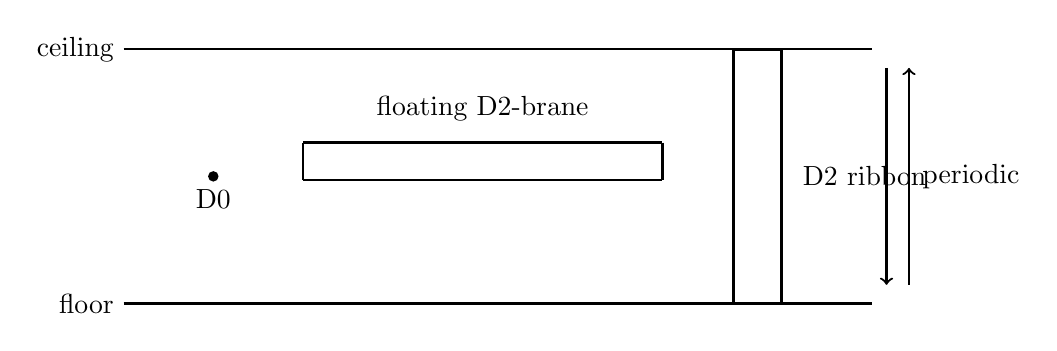
\begin{tikzpicture}[scale=0.95]
\draw[line width=0.9pt] (-5,1.7) -- (5,1.7);
\draw[line width=0.9pt] (-5,-1.7) -- (5,-1.7);

\node[left] at (-5,1.7) {ceiling};
\node[left] at (-5,-1.7) {floor};

\draw[->,line width=0.8pt] (5.2,1.45) -- (5.2,-1.45);
\draw[->,line width=0.8pt] (5.5,-1.45) -- (5.5,1.45);
\node[right] at (5.55,0) {periodic};

\draw[line width=1.0pt] (-2.6,0.45) -- (2.2,0.45);
\draw[line width=1.0pt] (-2.6,-0.05) -- (2.2,-0.05);
\draw[line width=1.0pt] (-2.6,0.45) -- (-2.6,-0.05);
\draw[line width=1.0pt] (2.2,0.45) -- (2.2,-0.05);
\node at (-0.2,0.9) {floating D2-brane};

\draw[line width=1.0pt] (3.15,-1.7) -- (3.8,-1.7);
\draw[line width=1.0pt] (3.15,1.7) -- (3.8,1.7);
\draw[line width=1.0pt] (3.15,-1.7) -- (3.15,1.7);
\draw[line width=1.0pt] (3.8,-1.7) -- (3.8,1.7);
\node[right] at (3.95,0) {D2 ribbon};

\fill (-3.8,0) circle (0.07);
\node[below] at (-3.8,-0.05) {D0};
\end{tikzpicture}
}%
\caption{샌드위치 콤팩트화. 위와 아래의 경계는 주기적으로 동일시된다. D2-브레인 하나는 카펫처럼 그 사이에 떠 있고, 또 하나는 바닥에서 천장까지 뻗어 있으며 콤팩트 방향이 작을 때는 끈처럼 보인다.}
\end{figure}

\subsection{D0-브레인과 D2-브레인은 어떻게 되는가?}

이제 강의는 D0-브레인과 끈에 무슨 일이 일어나는지 묻는다. 답은 서로 다르다. \(g\)가 커질수록 D0-브레인은 점점 가벼워진다. 고차원 해석에서는 새롭게 드러난 방향으로 운동량을 지닌 입자들의 탑에 합류한다. 따라서 약결합 그림에서 무겁고 복잡한 대상이 강결합 그림에서는 평범하고 가벼운 여기로 바뀐다.

질량 관계는 이러한 동일시를 보여준다.
\begin{equation}
M_{D0}(n)=\frac{n}{g_s\ell_s}
=\frac{n}{R_{11}}
=M_{\mathrm{KK}}(n).
\end{equation}
\editorialnote{서스킨드는 D0-브레인을 11차원 이론의 ``중력자''라고 부른다. 더 정확히는 이들의 결합 상태가 11차원 초중력 다중항의 칼루차--클라인 운동량 모드이며, 그 질량 없는 부문에 중력자가 포함된다. 이렇게 구분하면 강의에서 제시하는 물리적 동일성을 유지하면서 한 입자에 대한 문자 그대로의 과장된 진술은 피할 수 있다.}

D2-브레인은 끈의 운명을 설명한다. 강의에서 강조하는 배치는 두 가지다.
\begin{enumerate}
\item 땅콩버터 속 카펫처럼 바닥과 천장 사이에 떠 있는 D2-브레인,
\item 보이는 방향을 따라 뻗어 리본처럼 바닥에서 천장까지 이어진 D2-브레인.
\end{enumerate}샌드위치가 얇을 때 이 리본은 유효적으로 1차원처럼 보인다. 저에너지 관측자가 끈이라고 부르는 대상이 바로 이것이다. 콤팩트 방향이 열리면 같은 대상은 분명한 막의 형태를 띤다. 이제 수직 방향으로 더 많은 물질을 포함하므로 무거워지고 끈의 모습에서 멀어진다.

\paragraph{전이의 논리.}
\begin{enumerate}
\item 먼저 아주 작은 콤팩트 방향을 생각하자. 바닥에서 천장까지 이어진 리본은 사실상 끈처럼 거동한다.
\item \(g\)를 키우면 콤팩트 방향이 팽창한다.
\item 0-브레인은 가벼워져 고차원 이론의 칼루자--클라인 운동량 상태로 재해석된다.
\item 끈처럼 보이던 D2 리본은 눈에 띄게 펼쳐진 막이 되어 무거워진다.
\end{enumerate}
이 대목은 이중성에서 창발적 기하로 넘어가는 강의의 전환점이다. 강한 결합은 단순히 한 물체를 다른 물체로 바꾸는 데 그치지 않는다. 어느 기하가 더 효율적인지를 바꾼다.

Susskind는 이 설명이 얼마나 낯설게 들리는지 잠시 짚고 넘어간다. 제안된 여러 식별 관계가 성립하려면 까다로운 수학적 일관성 관계가 필요했으며, 그중 일부는 처음에는 물리학자들의 추측으로 제시되었다가 나중에 수학자들에 의해 증명되었다. 그의 주장은 모든 현실적인 끈 진공을 이해했다는 것이 아니라, 이중성의 연결망 자체가 이례적으로 엄격한 검증을 견뎌 왔다는 것이다.

이 이상화된 설정에서 결합상수가 위치에 따라 달라지면, 그에 따라 효율적인 기하도 달라질 수 있다. 한 영역은 가벼운 끈과 무거운 D0-브레인이 있는 거의 10차원 공간처럼 보일 수 있고, 다른 영역은 무거운 감긴 막과 가벼운 칼루자--클라인 모드가 있는 11차원 기술로 열릴 수 있다. 국소적으로 기술 방식이 달라지는 것도 같은 이중성 연결망의 일부다.

녹취록에는 이 관계의 이름이 ``부등식''으로 잠시 잘못 기록되어 있다. 문맥상 의도된 단어는 \emph{이중성}이다. 이는 매개변수 공간의 서로 반대쪽 끝을 잇는 관계를 뜻한다. 이 정정이 중요한 이유는 강의의 결론이 바로 근본 구성 요소의 유일한 목록은 알려져 있지 않다는 것이기 때문이다. 끈, 브레인, 입자, 고차원 기하는 서로 변환될 수 있다. 이 연결망에서 어느 구성원도 절대적으로 근본적이지 않거나, 아니면 더 깊은 구조가 아직 알려지지 않은 것이다.

\section{D3-브레인, 감긴 막, 그리고 이중성의 기하학적 그림}

휴식 후 Susskind는 이 주제를 서로 연결된 이론과 아이디어의 ``거대한 연결망''이라고 명시적으로 설명한다. 이어지는 예들은 각각 따로 떨어진 새로운 현상이 아니라, 앞서 나온 설명들을 서로 이어 주는 다리다.

\subsection{D3-브레인 월드볼륨}

첫 번째 다리에는 D3-브레인이 등장한다. D3-브레인은 공간 차원이 3개이므로, 그 위에 갇힌 관찰자는 그것을 평범한 공간으로 쉽게 오인할 수 있다. 브레인은 휘고 요동할 수 있으며, 브레인에 끝점을 둔 끈은 결합하거나 갈라지고 산란할 수 있다. 브레인 방향만 보는 관찰자에게 각 끝점은 입자로 보이고, 끝점들 사이의 상호작용은 보통의 양자장론처럼 보인다.

\begin{figure}[htbp]
\centering
\resizebox{\linewidth}{!}{%
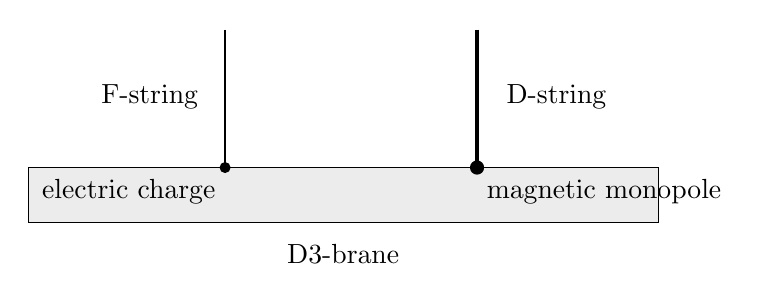
\begin{tikzpicture}[scale=1.0]
\draw[fill=gray!15] (-4,-0.35) rectangle (4,0.35);
\node at (0,-0.75) {D3-brane};

\draw[line width=0.9pt] (-1.5,2.1) -- (-1.5,0.35);
\fill (-1.5,0.35) circle (0.07);
\node[left] at (-1.72,1.25) {F-string};
\node[below left] at (-1.5,0.32) {electric charge};

\draw[line width=1.5pt] (1.7,2.1) -- (1.7,0.35);
\fill (1.7,0.35) circle (0.09);
\node[right] at (1.95,1.25) {D-string};
\node[below right] at (1.7,0.32) {magnetic monopole};
\end{tikzpicture}
}%
\caption{D3-브레인 월드볼륨 해석. F-끈의 끝점은 전하로 보이고, D-끈의 끝점은 자기 홀극으로 보인다.}
\end{figure}

이는 강의에서 가장 만족스러운 식별 관계 중 하나다. D3-브레인에 끝점을 둔 F-끈은 월드볼륨 관찰자에게 전하로 보인다. 같은 브레인에 끝점을 둔 D-끈은 자기 홀극으로 보인다. 다시 말해 F-끈과 D-끈 사이의 이중성은 D3-브레인 월드볼륨에서 보통의 장론에 나타나는 전기--자기 이중성이 된다. 앞서 비유였던 것이 이제 명시적인 대응표가 된다.

\editorialnote{D3-브레인 다발의 저에너지 월드볼륨 기술은 4차원 \(\mathcal N=4\) 초대칭 양--밀스 이론이다. 이 이론의 전기--자기 이중성은 IIB형 끈 이론의 S-이중성이 장론에서 구현된 것이다. 브레인 하나의 경우에는 강의에서 그림으로 사용한 아벨 극한에 해당한다.}

\subsection{두 콤팩트 방향과 비대칭 감기}

이어서 Susskind는 고차원 기하로 돌아가 작은 방향을 하나가 아니라 둘 콤팩트화한다. 11차원을 칠판에 그릴 수는 없으므로, 그림에 쓰이지 않는 큰 방향 일곱 개를 눈에 보이는 수평 방향 하나로 압축하고 두 콤팩트 방향은 따로 그린다. 그는 콤팩트화가 비대칭이 되도록 그려야 한다고 강조한다. 유효 끈들의 장력이 서로 다르려면 한 콤팩트 방향이 다른 방향보다 짧아야 하기 때문이다.

\begin{figure}[htbp]
\centering
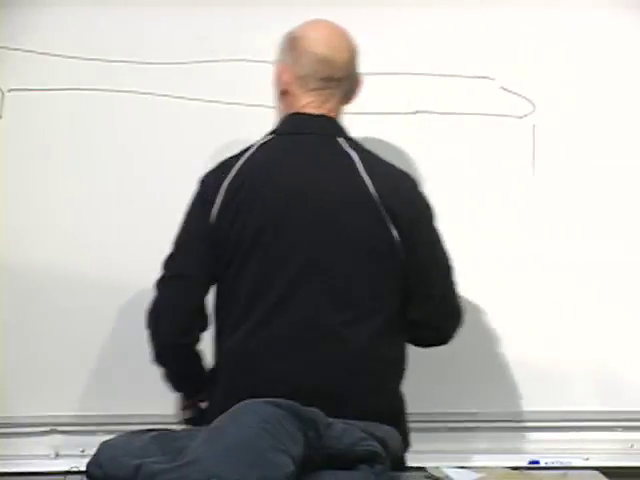
\includegraphics[width=0.78\textwidth]{lecture_01_figure_03.png}
\lectureframe{01:10:25.000}
\caption{두 감긴 막의 완성된 칠판 그림. 짧고 긴 콤팩트 주기가 오른쪽에 그려진 F-끈 및 D-끈 형태의 리본을 만든다.}
\end{figure}

막은 두 콤팩트 방향 중 어느 쪽으로든 감길 수 있으며, 비콤팩트 방향에서 보면 끈처럼 보인다. 두 원의 반지름이 \(R_1\)와 \(R_2\)라면 유효 장력은 다음과 같다.
\begin{equation}
\begin{aligned}
T_{(1)}&=2\pi R_1 T_{\mathrm{M2}},\\
T_{(2)}&=2\pi R_2 T_{\mathrm{M2}},\\
\frac{T_{(1)}}{T_{(2)}}&=\frac{R_1}{R_2}.
\end{aligned}
\end{equation}
따라서 원의 크기가 다르면 끈의 장력도 다르다. 더 짧은 방향으로 감긴 끈을 가벼운 F-끈으로, 더 긴 방향으로 감긴 끈을 무거운 D-끈으로 보면 개략적으로 다음과 같이 쓸 수 있다.
\begin{equation}
g_s\sim \frac{R_{\mathrm{short}}}{R_{\mathrm{long}}},
\qquad
\frac{T_{\mathrm{D1}}}{T_{\mathrm{F1}}}\sim \frac{1}{g_s}.
\end{equation}

\begin{classroomqa}
\audiencequestion{이 그림에서 결합상수를 두 콤팩트 차원의 비로 이해할 수 있습니까? \lecturetimestamp{01:10:13}}
\lecturerresponse{그렇다. 약--강 결합 매개변수는 종횡비로 기하학적으로 표현된다. 한 방향을 짧게 만들면 결합상수가 작아지고, 두 방향을 서로 맞바꾸면 가벼운 끈과 무거운 끈도 서로 바뀐다.}
\end{classroomqa}

\editorialnote{강의에서는 이 비를 잠시 \(\alpha\)라고 부르는데, 이는 앞서 양자전기역학의 미세구조상수를 나타낼 때 쓴 기호를 다시 사용한 것이다. 두 의미를 구별하기 위해 여기서는 \(g_s\)라고 쓴다. 완전한 M-이론 구성에서 IIB형 끈 이론의 결합상수는 콤팩트한 2차원 토러스의 복소구조에 담긴다. 분자의 정확한 형태는 토러스의 주기를 어떻게 이름 붙이느냐에 따라 달라진다.}

감긴 막의 그림은 칠판 그림의 원근 왜곡 없이 다음과 같이 요약할 수 있다.

\begin{figure}[htbp]
\centering
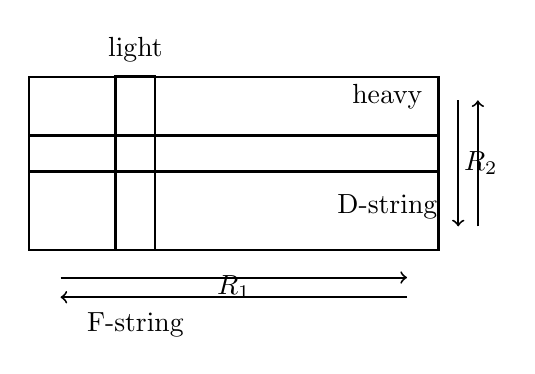
\begin{tikzpicture}[scale=1.0]
\draw[line width=0.9pt] (0,0) rectangle (5.2,2.2);
\node[below] at (2.6,-0.2) {\(R_1\)};
\node[right] at (5.4,1.1) {\(R_2\)};

\draw[->,line width=0.7pt] (5.45,1.9) -- (5.45,0.3);
\draw[->,line width=0.7pt] (5.7,0.3) -- (5.7,1.9);
\draw[->,line width=0.7pt] (0.4,-0.35) -- (4.8,-0.35);
\draw[->,line width=0.7pt] (4.8,-0.6) -- (0.4,-0.6);

\draw[line width=1.0pt] (1.1,0) -- (1.6,0) -- (1.6,2.2) -- (1.1,2.2) -- cycle;
\node at (1.35,2.55) {light};

\draw[line width=1.0pt] (0,1.45) -- (5.2,1.45);
\draw[line width=1.0pt] (0,1.00) -- (5.2,1.00);
\node at (4.55,1.95) {heavy};

\node at (1.35,-0.95) {F-string};
\node at (4.55,0.55) {D-string};
\end{tikzpicture}
\caption{감긴 막의 두 배치는 모두 비콤팩트 방향에서 끈처럼 보이지만, 콤팩트 방향의 크기가 다르면 한 유효 끈이 다른 끈보다 가벼워진다.}
\end{figure}

이는 앞서 살펴본 이중성 이야기의 기하학적 표현이다. 한 방향을 압축하는 동시에 다른 방향을 늘리면 감긴 물체 하나는 무거워지고 다른 하나는 가벼워져 F-끈과 D-끈의 역할이 서로 바뀔 수 있다.

\begin{classroomqa}
\audiencequestion{콤팩트 방향이 주기적이라면 감긴 물체는 폭이 무한합니까? \lecturetimestamp{01:10:41}}
\lecturerresponse{아니다. 콤팩트 원은 끝에 도달하지 않고 계속 돌 수 있지만 둘레는 유한하다. 잘라 펼친 그림의 위쪽과 아래쪽은 같은 점을 나타낸다. 구간의 양 끝점이 원의 한 점을 나타낼 수 있는 것과 같다.}
\end{classroomqa}

\begin{figure}[htbp]
\centering
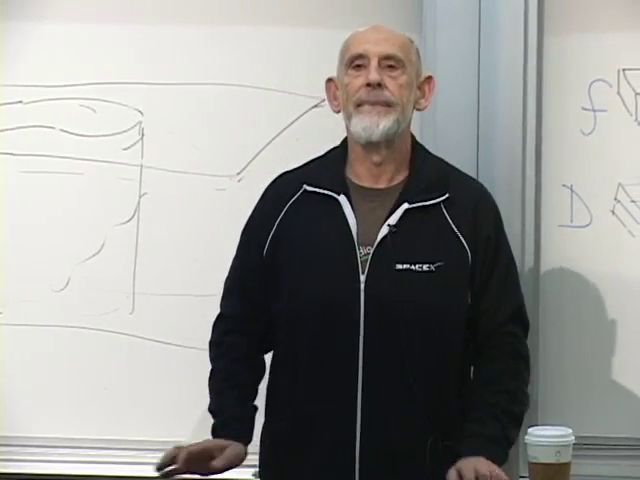
\includegraphics[width=0.78\textwidth]{lecture_01_figure_04.png}
\lectureframe{01:12:25.000}

\vspace{1em}

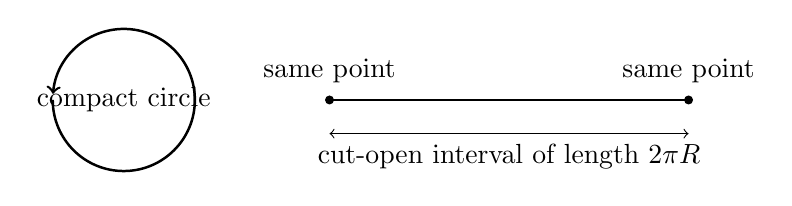
\begin{tikzpicture}[scale=0.95]
\draw[line width=0.9pt,->] (-3.7,0) arc[start angle=180,end angle=535,radius=0.95];
\node at (-2.75,0) {compact circle};
\draw[line width=0.9pt] (0.0,0) -- (4.8,0);
\fill (0.0,0) circle (0.06);
\fill (4.8,0) circle (0.06);
\draw[<->] (0.0,-0.45) -- (4.8,-0.45);
\node at (2.4,-0.75) {cut-open interval of length \(2\pi R\)};
\node[above] at (0.0,0.1) {same point};
\node[above] at (4.8,0.1) {same point};
\end{tikzpicture}
\caption{콤팩트 원과 그것을 칠판에서 잘라 펼쳐 나타낸 그림. 한쪽 끝점을 지나면 다른 쪽에서 이어진다. 원을 따라 움직이는 동시에 비콤팩트 방향으로도 이동하면 나선이 그려진다.}
\end{figure}

\begin{classroomqa}
\audiencequestion{콤팩트 경로는 왜 나선이 아니라 원입니까? \lecturetimestamp{01:12:23}}
\lecturerresponse{비콤팩트 방향의 각 고정된 점에서 콤팩트 방향은 원이다. 나선은 원을 따라 감기는 동시에 비콤팩트 방향으로 나아갈 때만 나타난다. 칠판의 구간은 단지 원을 잘라 펼친 것으로, 양 끝점은 서로 동일시된다.}
\end{classroomqa}

\begin{classroomqa}
\audiencequestion{이 기하 자체가 D-브레인을 가까이서 관측했을 때 F-끈들의 집합처럼 보이는 이유를 설명합니까? \lecturetimestamp{01:12:49}}
\lecturerresponse{둘 사이의 연결은 있지만, 이 기초적인 그림에서는 분명하게 드러나지 않는다. 이를 보려면 더 많은 기하학적 도구가 필요하다. 이 그림은 이중성을 정리하기 위한 것이지, 모든 미시적 구성 요소의 기술을 유도하기 위한 것은 아니다.}
\end{classroomqa}

\begin{classroomqa}
\audiencequestion{공간을 따라 이동하거나 시간이 흐르면서 긴 콤팩트 방향과 짧은 콤팩트 방향이 서로 바뀔 수 있습니까? \lecturetimestamp{01:13:35}}
\lecturerresponse{이상화된 모형에서는 둘 다 가능하다. 한 주기를 압축하고 다른 주기를 팽창시키면 어느 감긴 끈이 가벼운지가 바뀐다. 이것이 ``근본 끈''이란 명칭일 뿐인 또 하나의 이유다. 선호되는 기술 방식은 영역마다, 또는 시간에 따라 달라질 수 있다.}
\end{classroomqa}

\section{이상화, 특별히 대칭적인 점, 그리고 랜드스케이프}

강의의 마지막 부분에서 Susskind는 우아한 이중성의 예들에서 한 걸음 물러나, 그것들이 현실 세계에 대해 무엇을 말해 주며 무엇을 말해 주지 않는지 묻는다.

먼저 Susskind는 정밀하게 다룰 수 있는 이중성들이 보손과 페르미온의 질량이 정확히 일치하는 고도로 이상화된 초대칭 이론의 특징이라고 경고한다. 그는 뉴턴 역학의 원운동에 비유한다. 원운동은 대칭적이고 수학적으로 다루기 쉬우므로 먼저 연구하는 것이지, 실제 행성 운동이 완전한 원운동만으로 설명되기 때문은 아니다. 마찬가지로 초대칭 끈 이론은 자연보다 대칭성이 높아 분석하기 쉽다.

그렇다고 이상화가 유익하지 않은 것은 아니다. 완벽한 원운동은 현실적인 행성계는 아니지만, 대칭성이 낮은 궤도에서도 남아 있는 특징을 보여 준다. 마찬가지로 초대칭 사례들은 양자역학, 중력, 미시적 구조가 서로 모순 없이 결합할 수 있는 방식을 보여 준다. Susskind는 일부러 단호하게 말한다. 다루기 쉬운 끈 이론들은 문자 그대로 우리 세계의 이론이 아니다. 그 가치는 대칭성이 낮고 다루기 어려운 상황에서도 다시 나타날 가능성이 있는 현상을 드러낸다는 데 있다.

\subsection{여러 결과를 낳는 구성 도구}

D-브레인은 사용할 수 있는 구성 도구의 일부일 뿐이다. 강의에서는 플럭스, 오비폴드, 오리엔티폴드도 언급한다. 먼저 콤팩트 기하를 고른 다음, 어떤 브레인과 플럭스가 그 주기를 차지할지 선택한다. 간단한 샌드위치 모형조차 떠 있는 D2-브레인을 하나, 둘, 셋 넣느냐에 따라 저차원 물리가 달라진다. 이런 요소를 더하거나 빼면 유효 입자와 상호작용, 매개변수가 바뀐다.

강의에서 제시한 개략적인 수를 생각해 보자. 6차원 콤팩트 공간에 대략 \(500\)개의 주기가 있고, 각 주기에서 감긴 브레인이나 플럭스 또는 관련 구조를 고르는 방법이 대략 \(10\)가지라면, 구성의 수는 다음과 같이 증가한다.
\begin{equation}
N_{\mathrm{vacua}} \sim 10^{500}.
\end{equation}
강의의 계산 논리는 간단하다.
\begin{equation}
10 \times 10 \times \cdots \times 10 = 10^{500}
\end{equation}
여기서 인자는 \(500\)개다. DNA 비유를 들면 같은 점을 더 친숙한 방식으로 표현할 수 있다.
\begin{equation}
N_{\mathrm{DNA}}(500)=4^{500}.
\end{equation}
DNA를 비교하는 중에 청중 한 명이 한 가닥을 따라 가능한 선택지가 A, C, G, T 네 가지인지 확인한다. 이 정정은 주장을 바꾸지 않고 오히려 뒷받침한다. 몇 가지 국소적 선택을 여러 번 반복하면 전역적으로는 방대한 수의 배치가 생긴다. 정확한 지수가 핵심은 아니며, Susskind는 \(10^{500}\)이라는 수를 오래된 과소 추정치라고 부른다. 핵심은 조합론적 증식이다.

이로써 도입부에서 제기한 환원주의적 기대가 뒤집힌다. 복잡한 입자물리학이 반드시 복잡한 미시적 법칙에서 나오는 것은 아니다. 복잡한 유기체가 네 가지 염기로 이루어진 서열에 부호화될 수 있듯, 우리의 진공이 단순한 요소들을 복잡하게 배열한 결과일 수 있다.

\begin{classroomqa}
\audiencequestion{이중성으로 연결된 동등한 기술들을 하나로 묶고 나면, 완전한 정보가 가능한 진공들 가운데 우리 세계를 기술하는 하나 또는 몇 개만을 가려낼 수 있을까요? \lecturetimestamp{01:26:11}}
\lecturerresponse{아마도 제한된 집합을 골라낼 것이다. 하지만 서로 다른 여러 진공이 관측 가능한 에너지 범위에서는 매우 비슷해 보일 수 있다. 인용된 랜드스케이프의 수는 이중적인 기술을 하나로 묶은 뒤에도 여전히 크다는 뜻이다. 중요하지 않은 고에너지 세부 사항은 ``쓸모없는 DNA''}처럼 작용할 수도 있다.\end{classroomqa}

\subsection{대칭적인 점과 일반적인 복잡성}

랜드스케이프 안에는 특별히 대칭적인 점들이 있다. 기하학적 그림에서 두 방향의 종횡비가 같은 배치,
\begin{equation}
R_1=R_2,
\end{equation}
에서는 두 감긴 기술이 똑같이 단순해진다. 전기--자기 비유에서는 이를 개략적으로 다음과 같이 나타낸다.
\begin{equation}
m_{\mathrm{monopole}}=m_e.
\end{equation}

\begin{figure}[htbp]
\centering
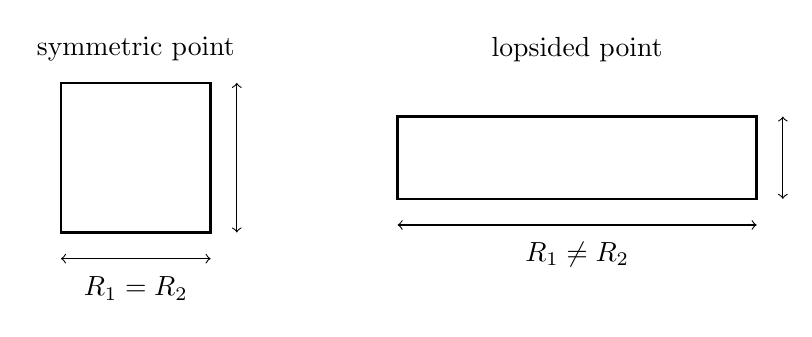
\begin{tikzpicture}[scale=0.95]
\draw[line width=0.9pt] (-4.5,-1.0) rectangle (-2.5,1.0);
\draw[<->] (-4.5,-1.35) -- (-2.5,-1.35);
\draw[<->] (-2.15,-1.0) -- (-2.15,1.0);
\node at (-3.5,1.45) {symmetric point};
\node at (-3.5,-1.75) {$R_1=R_2$};

\draw[line width=0.9pt] (0.0,-0.55) rectangle (4.8,0.55);
\draw[<->] (0.0,-0.9) -- (4.8,-0.9);
\draw[<->] (5.15,-0.55) -- (5.15,0.55);
\node at (2.4,1.45) {lopsided point};
\node at (2.4,-1.3) {$R_1\ne R_2$};
\end{tikzpicture}
\caption{종횡비가 같은 콤팩트화에서는 두 감긴 끈이 대칭적으로 다뤄진다. 한쪽으로 치우친 콤팩트화에서는 한 기술이 다른 기술보다 훨씬 가벼워진다.}
\end{figure}

\begin{classroomqa}
\audiencequestion{랜드스케이프에서 F-끈과 D-끈의 기술이 일치해 구성이 훨씬 단순해지는 진공도 있습니까? \lecturetimestamp{01:27:21}}
\lecturerresponse{그렇다. 특별히 대칭적인 점들이 있다. 우리 세계는 그중 하나에 있는 것으로 보이지 않는다. 익숙한 전기적 입자와 자기 홀극의 질량은 같지 않다. 자연이 한쪽으로 치우친 점에 놓인 이유는 알려져 있지 않다.}
\end{classroomqa}

\editorialnote{전자--홀극 질량이 같다는 것은 적절히 보호된 자기이중 모형에서 나타나는 개략적 특성이지, 보통의 비초대칭 양자전기역학이 예측하는 바가 아니다. 이는 관측된 전자에 관한 주장이 아니라 강의에서 말하는 대칭점의 개념을 표현한다.}

이어서 Susskind는 통신 이론의 비유를 든다. 무작위 부호는 놀라울 만큼 성능이 좋을 수 있지만, 기술하고 해독하기 쉬운 부호는 수학적 구조를 더 갖추고 있어 역사적으로 성능이 더 낮았다. 이후 부호 이론에서는 구조를 갖추면서도 매우 효과적인 구성이 발견되었지만, 비유의 요지는 여전히 유효하다. 간결한 이름이나 설명으로 나타낼 수 있는 것은 가능성 전체 공간에서 복잡도가 낮은 매우 특별한 부분에 속한다. 마찬가지로 계산하기 가장 쉬운 끈 진공은 전형적이지 않을 수 있다.

따라서 적절한 질문도 달라질 수 있다. 미시적 세부 사항까지 모두 포함한 정확한 콤팩트화를 요구하는 대신, 폭넓은 앙상블에서 어떤 특징이 공통적이거나 일반적인지 물을 수 있다. Susskind는 이를 확정된 결론이 아니라 연구 과제로 제시하며, 계산 대신 이념적 주장을 내세우는 것을 거부한다.

\subsection{우주론적 질문}

\begin{classroomqa}
\audiencequestion{둘레가 엄청나게 큰 콤팩트 방향은 무한한 방향과 관측상 구별됩니까? 우리에게 큰 공간 차원이 3개 있다는 것은 알지만, 그 차원들이 무한하다는 것도 알고 있습니까? \lecturetimestamp{01:30:03}}
\lecturerresponse{그 차원들이 무한하다는 사실은 알지 못한다. 닫힌 3차원 구면은 콤팩트한 채로 팽창할 수 있다. 거의 평평하다는 측정 결과는 곡률 반지름의 하한만 제공한다. 거의 평평한 들판을 측량해 지구의 크기에 상한을 둘 수는 있어도, 지구 표면이 무한하다는 것을 증명할 수는 없는 것과 같다. 유한한 규모를 결정하려면 곡률을 검출하거나 전역적 동일시를 확인해야 한다.}
\end{classroomqa}

\begin{classroomqa}
\audiencequestion{이상화된 모형에서 결합 상수가 공간에 따라 달라질 수 있다면, 현실 세계에서는 그런 변화가 어떻게 일어날 수 있을까요? \lecturetimestamp{01:32:43}}
\lecturerresponse{대칭적인 예에서 사용한 것처럼 제한 없이 연속적으로 변하는 방식으로는 일어나지 않습니다. 뒤에서 논의할 현실적인 가능성은 서로 다른 유효 법칙을 따르는 영역들 사이의 이산적 전이를 통해 변하는 것입니다. 그런 도약이 일어나는지는 우주론의 문제입니다.}
\end{classroomqa}

\editorialnote{이 답변은 모든 스칼라장이 매끄럽게 변할 수 없다는 일반 정리가 아니라, 플럭스 진공과 영역 전이에 대한 강의의 예고로 읽어야 한다. 관측은 무차원 결합상수의 변화를 강하게 제한하며, 주어진 모형에서 연속적인 모듈라이가 남아 있는지는 안정화 메커니즘에 달려 있다.}

녹음에는 마지막 청중 질문이 남아 있지 않다. 보존된 답변에 따르면 제안된 현상은 일부 종류의 블랙홀에서는 일어날 수 있지만, 자유 낙하 관찰자에게 국소적으로 평범한 장소인 보통의 슈바르츠실트 블랙홀 지평선에서는 일어나지 않는다. 질문 내용을 신뢰성 있게 복원할 수 없으므로, 이 대화에 더 구체적인 주장을 덧붙이지 않는다.

\section{벽돌에서 기술의 연결망으로}

물리학의 더 깊은 층위는 반드시 더 단순해야 한다는 기대는 취약한 것으로 드러났다. \(1+1\)차원 보손화에서는 같은 이론을 페르미온 중심으로 구성할 수도 있고 보손 중심으로 구성할 수도 있으며, 이때 페르미온은 킨크로 다시 나타난다. 양자전기역학에서는 약결합과 강결합에 따라 전자와 자기 홀극의 기술상 역할이 서로 바뀐다. 끈 이론에서는 F-끈과 D-끈이 같은 양상을 되풀이한다. 브레인이 짝수 개인 이론에서는 강결합이 한 걸음 더 나아간다. 콤팩트 방향이 팽창하고, D0-브레인은 칼루자--클라인 운동량 상태가 되며, 유효 끈은 고차원 기하에서 감긴 막으로 재해석된다. 따라서 현대 양자장론과 끈 이론은 ``어느 것이 벽돌이고 어느 것이 집인가?''라는 질문에 단번에 고정된 유일한 답을 주지 않는다. 각 기술이 자기 영역에서 효율적인 기술들의 연결망과, 일반적인 결과가 단순함보다 복잡성인 방대한 가능성의 랜드스케이프를 제시한다.
